\documentclass{beamer}
\usetheme[pageofpages=of,% String used between the current page and the
                         % total page count.
          bullet=circle,% Use circles instead of squares for bullets.
          titleline=true,% Show a line below the frame title.
          alternativetitlepage=true,% Use the fancy title page.
       %   titlepagelogo=logo-polito,% Logo for the first page.
       %   watermark=watermark-polito,% Watermark used in every page.
       %   watermarkheight=100px,% Height of the watermark.
       %   watermarkheightmult=4,% The watermark image is 4 times bigger
                                % than watermarkheight.
          ]{Torino}

\setbeamertemplate{footline}{
  \begin{beamercolorbox}[wd=\paperwidth,ht=1ex,dp=1ex]{footline}
    \vspace{5pt} \hspace{1em} \insertframenumber/\inserttotalframenumber
  \end{beamercolorbox}
}

\newcommand{\given}{\,|\,}

\usepackage{colortbl}
\definecolor{LightGray}{gray}{0.9}
\definecolor{DarkGray}{gray}{0.3}
\definecolor{LightCyan}{rgb}{0.9, 1, 1}
\definecolor{LightRed}{rgb}{1, 0.8, 0.8}
\definecolor{LightGreen}{rgb}{0.8, 1, 0.8}
\definecolor{DarkGreen}{rgb}{0.3, 0.5, 0.3}



\author{Brendon J. Brewer}
\title{Introduction to Bayesian Statistics}
\institute{Summer Institute in Statistical Genomics \\
The University of Auckland, November 2026}
\date{}


\linespread{1.3}
\usepackage{minted}
\usepackage[utf8]{inputenc}
\usepackage{dsfont}


\begin{document}

\frame{\titlepage}


\begin{frame}
\begin{center}
\Large
Introduction to MCMC
\end{center}

\end{frame}

\begin{frame}
\frametitle{Philosophy}
\begin{itemize}
\item Markov Chain Monte Carlo (MCMC) algorithms are, strictly speaking, not
Bayesian.\pause
\item However, they are associated with Bayesian statistics because they happen
to be very useful in this area.\pause
\item They allow us to describe posterior distributions in more than one
dimension (more than one unknown parameter) quite easily.
\end{itemize}
\end{frame}

\begin{frame}
\frametitle{More Than One Parameter}
So far we have focused on single-parameter problems until we get used to the
Bayesian approach. But most real problems have more than one unknown parameter.
Imagine making a Bayes Box:
\begin{center}
{\tiny
\begin{tabular}{|c|c|c|c|c|}
\hline
Parameter & Prior & Likelihood & Prior $\times$ Likelihood & Posterior \\
$(\theta_1, \theta_2)$  & $p(\theta_1, \theta_2)$ & $p(x \given \theta_1, \theta_2)$ & $p(\theta_1, \theta_2)p(x\given\theta_1, \theta_2)$ & $p(\theta_1, \theta_2\given x)$ \\
\hline
(0, 0) &  &  & & \\
(0, 0.1) &  &  & & \\
... & ... & ... & ... & ... \\
(0.1, 0) &  &  & & \\
(0.1, 0.1) & & & & \\
... & ... & ... & ... & ... \\
(1, 0.9) & & & & \\
(1, 1) & & & & \\
\hline
Total & 1 & & & 1 \\
\hline
\end{tabular}
} % tiny
\end{center}

\end{frame}

\begin{frame}
\frametitle{More Than One Parameter}
\begin{itemize}
\item Because each hypothesis is about the value of the {\em pair}
$(\theta_1, \theta_2)$, instead of say 100 grid points, we would need
100 $\times$~100. \pause
\item This is quite feasible, but annoying, because you would need 2D arrays
instead of vectors.\pause
\item However, in even higher dimensions (let's say 100) you would need
$10^{100}$ rows (or something like that) in your Bayes Box.
That is not going to happen.
\end{itemize}


\end{frame}


\begin{frame}[fragile]
\frametitle{Grids vs. Samples}
\begin{itemize}
\item You can think of the grid-based approach, which we have used so far,
as assigning {\bf weights} to the $\theta$ values. The posterior probabilities
are the weights, which is why you do calculations like
\mintinline{r}{sum(theta*post)} to get the posterior mean.\pause
\item The purpose of MCMC is to generate {\bf samples} from the posterior
distribution. This is a collection of $\theta$ values that implicitly have
equal weight. To get the posterior mean you would just do \mintinline{r}{mean(theta)}.
This is called {\bf Monte Carlo}.
\end{itemize}


\end{frame}


\begin{frame}[fragile]
\frametitle{Grids vs. Samples}
\centering
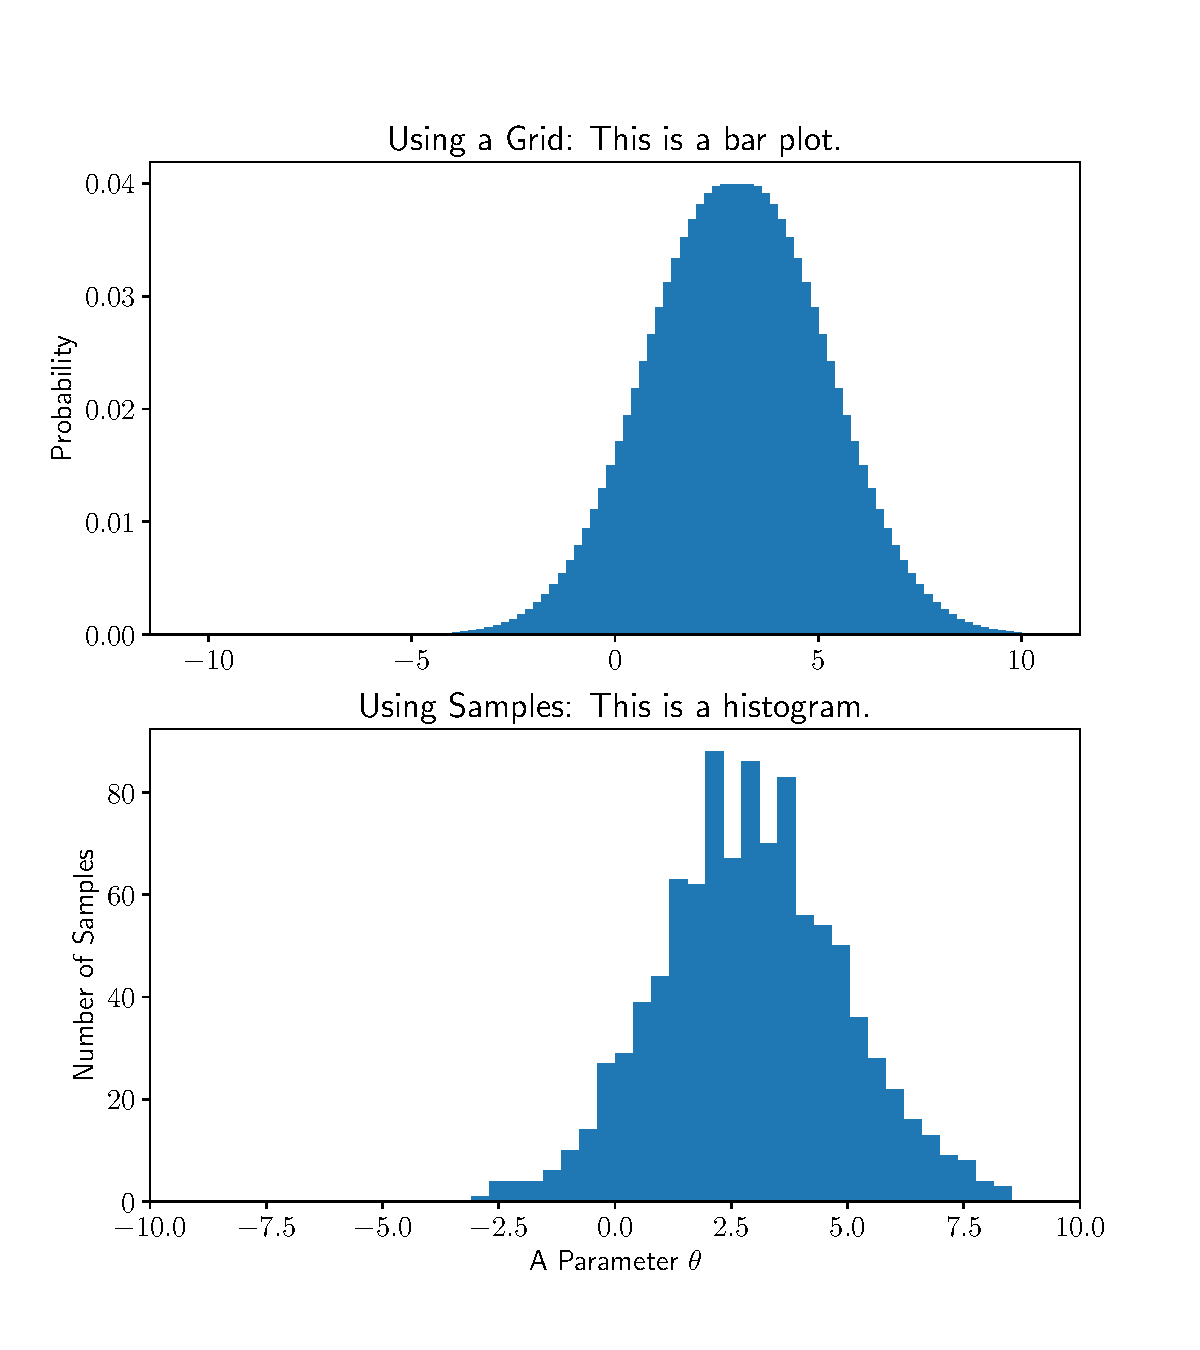
\includegraphics[width=0.6\textwidth]{images/grid_vs_samples.pdf}

\end{frame}

\begin{frame}
\frametitle{Using Monte Carlo Samples}
\begin{itemize}
\item If we can generate random numbers from the
posterior, then the histogram will look just like the posterior.\pause
\item If we have enough random numbers, we can use the
sample mean which will be almost the same as the
actual posterior mean.\pause
\item Same with sd or any other summary.
\end{itemize}

\end{frame}

\begin{frame}
\frametitle{Monte Carlo}
\centering
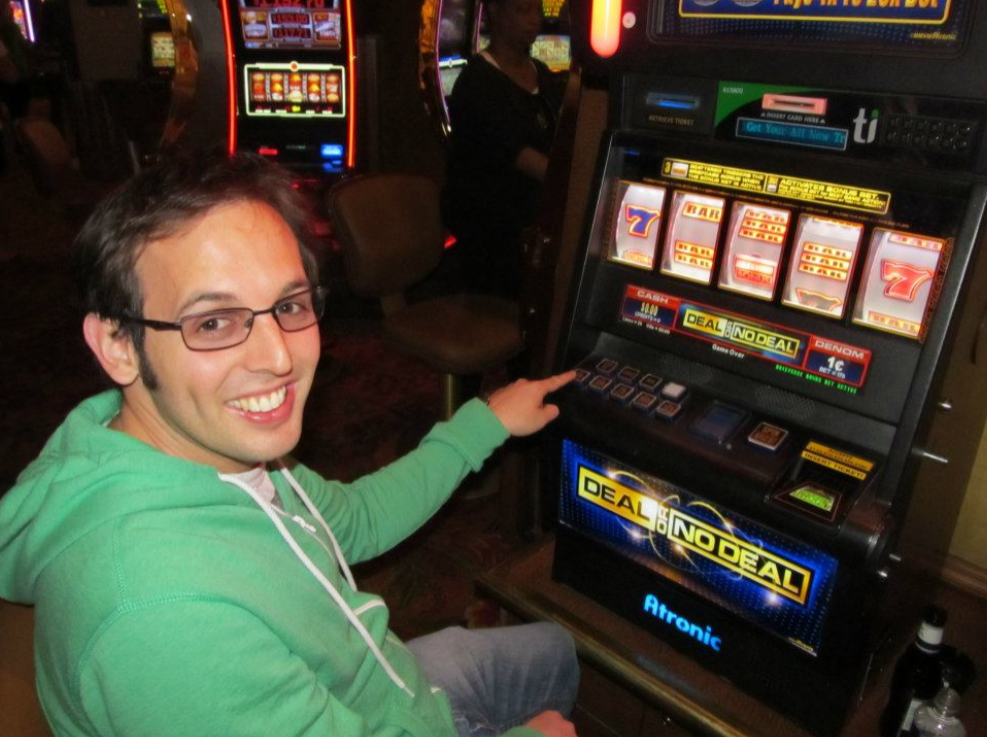
\includegraphics[width=0.6\textwidth]{images/vegas.png}

I was actually in Las Vegas, not Monte Carlo.

\end{frame}

\begin{frame}
\frametitle{Large Sample Size}

\begin{itemize}
\item More samples means the generated $\theta$ values more accurately
reflect the posterior.\pause
\item But the posterior still has the uncertainty built into it, as represented
by the scatter in the generated $\theta$ values.\pause
\item We will assume that we always have a `large enough'
sample from the posterior. It is possible to worry about extra
uncertainty from the Monte Carlo approximation itself, but we will ignore this.
\end{itemize}

\end{frame}



\begin{frame}
\frametitle{Marginalisation}
Marginalisation is the process of going from a higher dimensional probability
distribution to a lower dimensional one. Consider the following table,
with a parameter $\theta_1$ on the $x$-axis and $\theta_2$ on the $y$-axis.
\begin{align}
\begin{array}{c|cccc}
4 & 1/16 & 1/12 & 1/8 & 1/4 \\
3 & 1/16 & 1/12 & 1/8 & 0 \\
2 & 1/16 & 1/12 & 0   & 0 \\
1 & 1/16 & 0    & 0   & 0 \\
\hline
  & 1    & 2    & 3   & 4
\end{array}
\end{align}
\pause
If we only really care about $\theta_1$, we sum the columns
to get the {\bf marginal distribution}.


\end{frame}


\begin{frame}
\frametitle{Marginalisation}
The result of the marginalisation is the following probability distribution
for $\theta_1$ by itself:

\begin{center}
\begin{align}
\left\{\frac{1}{4}, \frac{1}{4}, \frac{1}{4}, \frac{1}{4}\right\}
\end{align}
\end{center}

\end{frame}


\begin{frame}
\frametitle{General Marginalisation}
If there are parameters $\theta_1, ..., \theta_N$ that we care about,
and ``nuisance parameters'' $\phi_1, ..., \phi_M$ that we don't, we can
{\bf integrate out} the nuisance parameters (this is similar to the column
sum we just did).
\pause
\begin{align}
p(\theta_1, ..., \theta_N \given x)
    &= \int p(\theta_1, ..., \theta_N, \phi_1, ..., \phi_M \given x)
            \, d\phi_1 ... d\phi_M.
\end{align}
\pause
One of the benefits of Monte Carlo is that we can avoid doing this integral.
\end{frame}



\begin{frame}
\frametitle{Marginalisation}
\centering
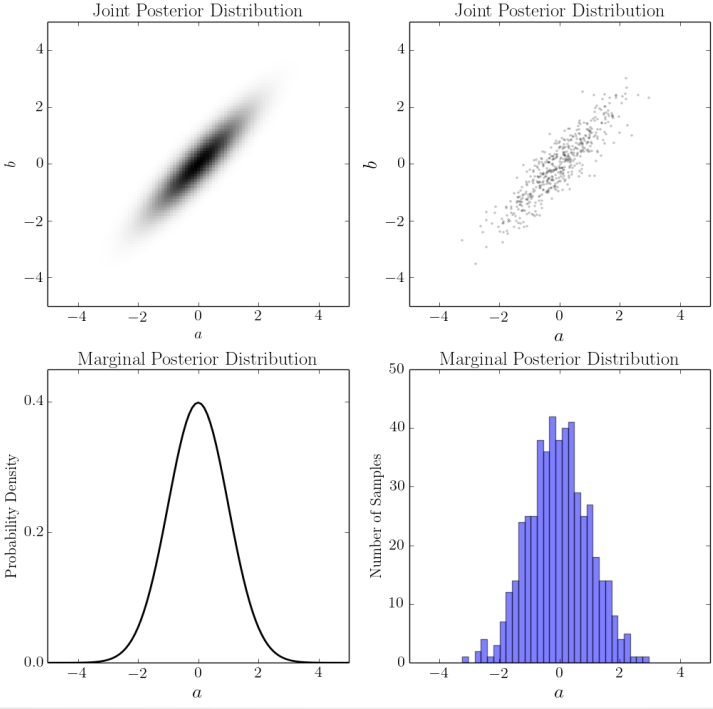
\includegraphics[width=0.6\textwidth]{images/marginalisation.png}

\end{frame}

\begin{frame}
\frametitle{Marginalisation}
Our samples will usually be in a 2D array format (or an R data frame),
where each row is one sample from the joint posterior and each column is
a particular parameter.
To get a marginal distribution we simply look at one column at a time.
This is a lot easier than multiple integration!

\end{frame}


\begin{frame}
\frametitle{Markov Chain}
{\bf Monte Carlo} is about the use of samples to approximate a probability
distribution (for us, almost always the posterior distribution). Markov chains
are used when we actually generate the samples.
\pause

A Markov Chain is sequence of `random variables', where each one
depends on the previous one but not on the ones before that.
A general joint distribution:
\begin{align}
p(x_1, x_2, x_3, x_4) &= p(x_1)p(x_2 \given x_1)p(x_3 \given x_2, x_1)
                    p(x_4 \given x_3, x_2, x_1)
\end{align}
A Markov Chain:
\begin{align}
p(x_1, x_2, x_3, x_4) &= p(x_1)p(x_2 \given x_1)p(x_3 \given x_2)p(x_4 \given x_3).
\end{align}


\end{frame}


\begin{frame}
\frametitle{An Example Markov Chain}
A {\bf random walk} is an example of a Markov Chain.

\begin{itemize}
\item Start at position $x=0$.\pause
\item Flip a coin.\pause
\item Heads? Add 1. Tails? Subtract 1.\pause
\end{itemize}

You will get a sequence like this:
0, -1, 0, 1, 2, 3, 2, 1, 2, 3, 4, 3, 4, ...
\pause

The thing that is a Markov Chain is the probability distribution for the
sequence, not a given sequence itself.

\end{frame}

\begin{frame}
\frametitle{Markov Chains: Stationary Distribution}
Markov Chains often have a {\bf stationary distribution}.

\begin{itemize}
\item If you start with an initial point specified probabilistically
with the stationary distribution, then the distribution for `where I go next'
is also the stationary distribution.\pause
\item It is the probability distribution representing where the
algorithm will be after a long time.\pause
\item With high probability, it is also the
frequency distribution of results you get
after running the chain for a long time.
\end{itemize}


\end{frame}

\begin{frame}
\frametitle{MCMC Target Distributions}
The key idea of MCMC is to engineer a Markov Chain whose stationary distribution
is the {\bf target distribution} that you are interested in --- for us, this
will mostly be a posterior distribution. There are a few different ways to do
this. We will study the {\bf Metropolis algorithm}.

\end{frame}




\begin{frame}
\frametitle{The Metropolis Algorithm}
The {\bf Metropolis Algorithm} (sometimes {\bf Metropolis-Hastings})
is one of the most famous and general
MCMC methods available, invented in the 1950s. The output looks like a Metropolis:
\begin{center}
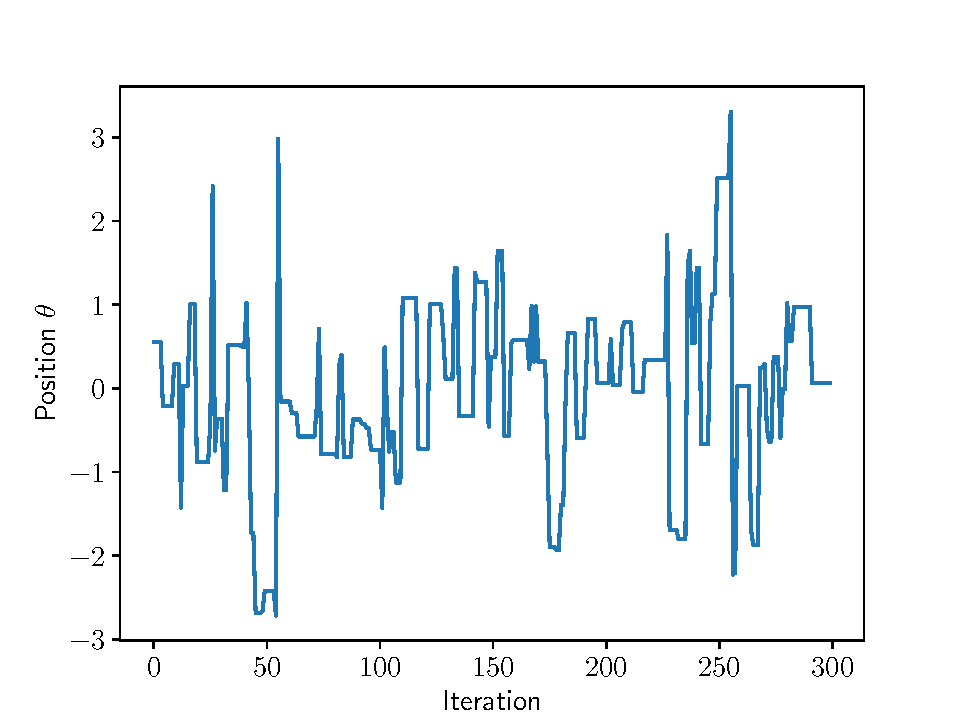
\includegraphics[width=0.6\textwidth]{images/metropolis.pdf}
\end{center}

\end{frame}

\begin{frame}
\frametitle{The Metropolis Algorithm}
That is just a coincidence.
It is actually named after Nicholas Metropolis.

\begin{center}
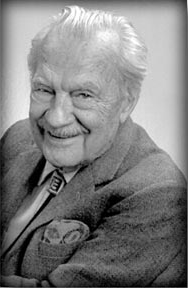
\includegraphics[width=0.2\textwidth]{images/nicholas_metropolis.png}

(Public domain image)
\end{center}

\end{frame}


\begin{frame}
\frametitle{The Metropolis Algorithm}
\begin{itemize}
\item We want to sample the posterior distribution for a Bayesian inference problem. \pause
\item Start with something we {\em can} do, called the {\bf proposal distribution.}\pause
\item Use {\bf acceptance and rejection} to modify the distribution into the
one we want.\pause
\item To implement Metropolis, we assume that a function exists which returns
the prior times likelihood value for whatever value of parameters $\theta$
we pass in.
\end{itemize}

\end{frame}

\begin{frame}
\frametitle{An Example Proposal Distribution}

\begin{itemize}
\item As a simple example, suppose $\theta \in \{1, 2, 3, 4, 5\}$, and our proposal
distribution is a wrapped random walk (so if you are at 5 and you try to add
one, it wraps back to 1).\pause
\item If we let this happen for a long time, we will end up with a uniform
(frequency) distribution of $\theta$ values, because that is the
{\bf stationary distribution} of this Markov Chain.\pause
\item Putting in acceptance and rejection modifies the stationary distribution
of the Markov Chain so that it becomes the target distribution of interest
(the posterior).
\end{itemize}

\end{frame}


\begin{frame}
\frametitle{Acceptance and Rejection}
\centering
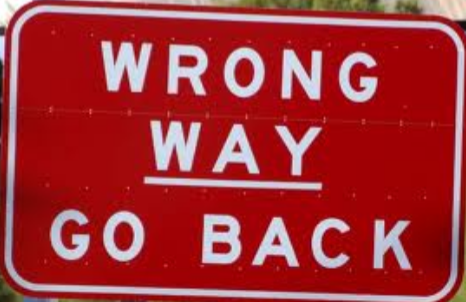
\includegraphics[width=0.7\textwidth]{images/wrong_way.png}

\end{frame}

\begin{frame}
\frametitle{Acceptance and Rejection}
Call the prior times likelihood function $h(\theta)$.
If we try to move from $\theta$ to $\theta'$ because the proposal distribution
resulted in $\theta'$, we only accept it with the following probability:
\begin{align}
P(\textnormal{accept}) &= \min\left(1, \frac{h(\theta')}{h(\theta)}\right)
\end{align}
\pause

That is, uphill moves are accepted. Downhill moves are accepted with a probability
based on the ratio of prior $\times$ likelihood values.

\end{frame}


\begin{frame}[fragile]
\frametitle{Trace Plots}
A {\bf trace plot} is simply a plot of a parameter over time as the MCMC
proceeds. If the results are in a vector called \mintinline{r}{keep}, they are easy to produce:
\begin{minted}{r}
plot(keep, type="l", xlab="Iteration", ylab="theta")
\end{minted}

\end{frame}

\begin{frame}[fragile]
\frametitle{An Example Trace Plot}
This is what a trace plot looks like when things are working well.

\begin{center}
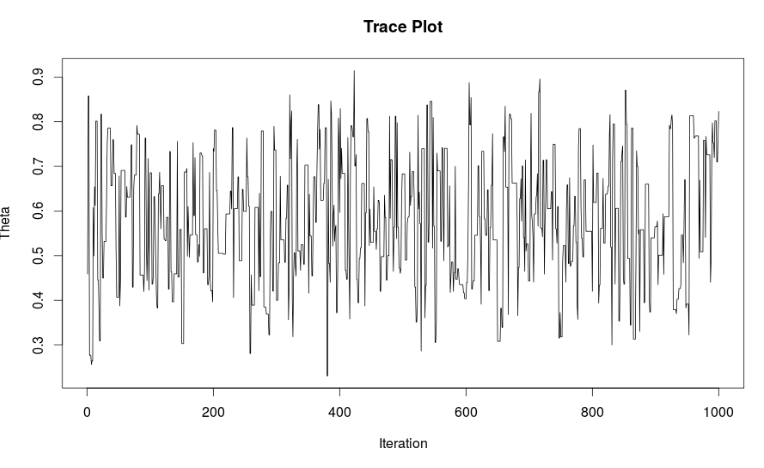
\includegraphics[width=0.8\textwidth]{images/trace_plot.png}
\end{center}

Some people call it a ``fuzzy caterpillar''.

\end{frame}





\begin{frame}
\frametitle{Running MCMC}
MCMC does not always work perfectly. There are several phenomena
we should look for:
\begin{itemize}
\item `Burn-in', which occurs when the starting point is not in a typical region
of the target/posterior distribution.\pause
\item Poor mixing, which can occur when the posterior distribution
has a difficult structure.
\end{itemize}

\pause
These can usually be diagnosed with trace plots.

\end{frame}




\begin{frame}
\frametitle{Introduction to JAGS}

\begin{itemize}
\item JAGS is a general purpose computer program for doing
MCMC sampling.\pause
\item It is useful for routine analyses (less useful for very large or
research problems).\pause
\item You tell it the prior, the sampling distribution, and the data and it will
do everything for you!\pause
\item It uses methods other than Metropolis (Gibbs sampling,
slice sampling, ...).
\end{itemize}

\end{frame}


\begin{frame}
\frametitle{Alternatives to JAGS}

There are some other programs similar to JAGS. I will mention them here,
so that you've heard of them, but we will not use them in this course.

\begin{itemize}
\item WinBUGS and OpenBUGS are both very similar to JAGS (the former is very
old and only works on Microsoft Windows).
Most of the time, code would not need to be modified to work in any of these.\pause
\item {\bf Stan} is a more modern and very popular package. It uses similar
ideas to JAGS, but its language is a bit different, and it uses a different,
more complex
MCMC sampler (based on {\bf Hamiltonian Monte Carlo}).
\end{itemize}

\end{frame}

\begin{frame}[fragile]
\frametitle{Installing JAGS}
You can install JAGS by first downloading it from this URL. Install it to
the default location on your system to avoid problems later.

\begin{center}
\url{https://mcmc-jags.sourceforge.io/}
\end{center}

\pause

After installing JAGS itself, you should install the \mintinline{r}{rjags}
package inside R:
\begin{minted}{r}
install.packages("rjags")
\end{minted}

\end{frame}


\begin{frame}[fragile]
\frametitle{The Bus Problem}
Recall the bus problem from the lecture notes. This was a binomial experiment
with $N=5$ trials, and the data was $x=2$ successes. The unknown parameter
is $\theta$, the success probability that applies on each trial.

\pause

We know how to solve this with a grid (Bayes Box), analytically (with a Beta
or Uniform prior for $\theta$), and with Metropolis.
How would we implement this in JAGS?

\end{frame}


\begin{frame}[fragile]
\frametitle{The Bus Problem in JAGS}

\begin{minted}{r}
model
{
    # The prior for the parameter
    theta ~ dunif(0, 1)

    # Sampling distribution (prior for the data!)
    x ~ dbin(theta, N)
}
\end{minted}

\end{frame}

\begin{frame}[fragile]
\frametitle{The Bus Problem in JAGS}
\begin{itemize}
\item We always write the assumptions inside the \mintinline{r}{model} block.\pause
\item We generally put the prior before the sampling distribution, but we don't
    actually have to!\pause
\item Quantities (either parameters or data) are defined into existence using
the tilde \mintinline{r}{~}.\pause
\item Note that $N$ is not defined anywhere --- this will be provided along
with the data value $x$.
\end{itemize}

\end{frame}

\begin{frame}[fragile]
\frametitle{Note About dbin() in JAGS}

\begin{itemize}
\item The distributions in JAGS are named similarly to the \mintinline{r}{d}
(density) functions in R, but not exactly the same --- here we see
\mintinline{r}{dbin()} whereas in R it's \mintinline{r}{dbinom()}.\pause
\item Also, people usually write Binomial$(N, p)$ or Binomial$(N, \theta)$,
but in JAGS the arguments are the other way around.\pause
\item There are some other quirks. E.g., for the normal distribution, the
second argument is {\em one over the variance}, i.e., we must write
\mintinline{r}{dnorm(mu, 1/sigma^2)}. 
We could write \mintinline{r}{dnorm(mu, 5)}
but the meaning of the second parameter is obscured.
\end{itemize}

\end{frame}



\begin{frame}[fragile]
\frametitle{Running JAGS from R}

\begin{itemize}
\item We will write R code that calls JAGS in the background using functions
from the \mintinline{r}{rjags} package.\pause
\item There is a script on Canvas called \texttt{use\_jags.R} which you can
use as a template.\pause
\item The JAGS model code is provided inside an R string.\pause
\item The data must be in an R list or data frame.\pause
\item After running the script, the results are put into a data frame called
\mintinline{r}{results}, whose (named) columns are the parameters.
\end{itemize}

\end{frame}




\begin{frame}[fragile]
\frametitle{Running JAGS on the Bus Problem}
Let's run JAGS on the bus problem. We will need to ``monitor''
\mintinline{r}{theta}, by including it in the \mintinline{r}{variable_names}
vector, if we want to see it in the output.

\end{frame}



\begin{frame}[fragile]
\frametitle{Visualisation and Summaries}
It is easy to visualise and summarise the posterior:

\begin{minted}{r}
plot(results$theta, type=”l”)
hist(results$theta, breaks=100)
mean(results$theta)
sd(results$theta)
\end{minted}

\end{frame}



\begin{frame}[fragile]
\frametitle{Coal Data}

\centering
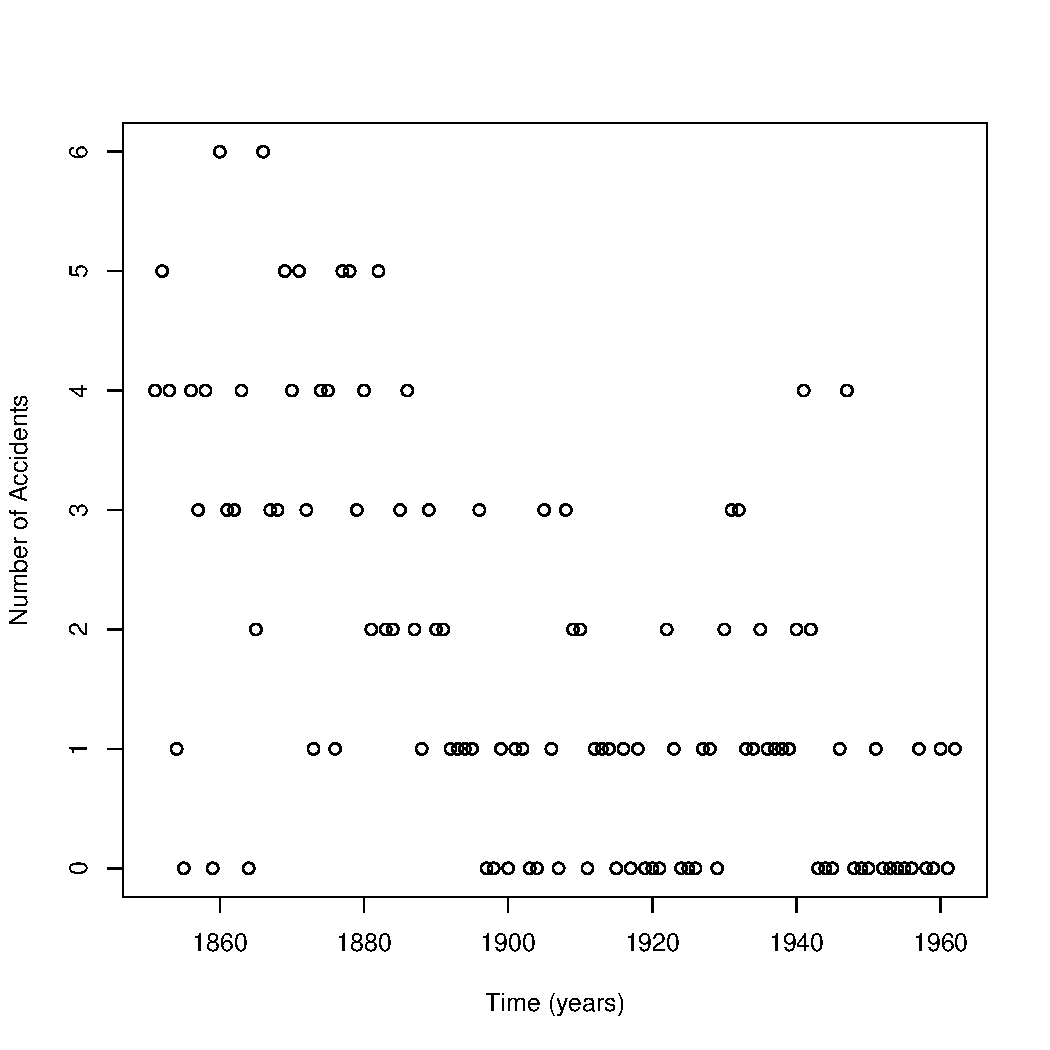
\includegraphics[width=0.6\textwidth]{images/coal.pdf}

\end{frame}


\begin{frame}[fragile]
\frametitle{Coal Data}
The coal mining data is in a .R file that just defines a list.
We need to ``source'' the file --- run all the code in it. We can just
click source in RStudio, or we can use the \mintinline{r}{source()}
function to do it:
\begin{minted}{r}
source("coal.R")
\end{minted}
\pause
We may need to put the full file path in the argument, or change
R's working directory.

\end{frame}




\begin{frame}[fragile]
\frametitle{Coal Mining Accidents --- Simple Model}

\begin{minted}{r}
model
{
    # Somewhat arbitrary upper limit
    lambda ~ dunif(0, 1000)

    for(i in 1:N) # For-loop syntax is like R
    {
        y[i] ~ dpois(lambda)
    }
}
\end{minted}

\end{frame}


\begin{frame}[fragile]
\frametitle{Coal Mining Accidents --- For Loop}
\begin{itemize}
\item The sampling distribution involves a loop because we have a vector
of data values.\pause
\item This is usually what happens, but not always --- it is possible to
put parameters in a vector too, if you want.\pause
\item The for-loop syntax is very similar to R's for loops.\pause
\item \mintinline{r}{N}, the number of data points, is defined in the
data list. We could also use \mintinline{r}{for(i in 1:length(y))} or
\mintinline{r}{for(i in 1:length(t))}.
\end{itemize}

\end{frame}


\begin{frame}[fragile]
\frametitle{Coal Mining Accidents --- Results}
Let's run \texttt{use\_jags.R} and look at the results.

\end{frame}



\begin{frame}
\frametitle{Coal Mining Accidents --- Log-Uniform Prior}
We will now see how to define a log-uniform prior in JAGS,
as an alternative to the Uniform$(0, 1000)$ prior that we have
seen so far. Remember, there are two ways of defining the
log-uniform prior:\pause
\begin{align}
p(\lambda) &\propto 1/\lambda, \quad \lambda > 0
\end{align}
\pause
or
\begin{align}
\log \lambda &\sim \textnormal{Uniform}(-\infty, \infty).
\end{align}
\pause
JAGS doesn't allow infinite range (an `improper' prior),
but we can just use a wide range.

\end{frame}


\begin{frame}[fragile]
\frametitle{Coal Mining Accidents --- Log-Uniform Prior}
To define a log-uniform prior in JAGS, we can use two lines of code.
\begin{minted}{r}
log_lambda ~ dunif(-10, 10)
lambda <- exp(log_lambda)
\end{minted}
\pause

The first line creates a parameter with a uniform prior. If
we exponentiate it, the result has a log-uniform prior.\pause

The range is from $e^{-10} \approx 0.000045$ to $e^{10} \approx 22000$,
which is wide enough for most purposes. Not astronomy though!
\end{frame}


\begin{frame}[fragile]
\frametitle{Deterministic and Stochastic Nodes}
\begin{itemize}
\item The parameter \mintinline{r}{lambda} was defined using \mintinline{r}{<-}
using an equation, not a probability distribution. Because an equation always
gives a definite answer, this is called a {\em deterministic node}. \pause
\item You can also use \mintinline{r}{=} these days.\pause
\item Quantities defined using \mintinline{r}{~} and a probability distribution,
whether they are parameters or data values, are called
{\em stochastic nodes}.
\end{itemize}
\end{frame}


\begin{frame}[fragile]
\frametitle{Coal Mining Accidents --- ChangePoint Model}
We will now make a more complicated model, to show the power of JAGS and
MCMC. It will be a
``change-point'' model, where instead of having a
constant $\lambda$ value, we assume it changes from
$\lambda_1$ to $\lambda_2$ at some critical time $t_c$.
These are the three unknown parameters.

Looking at the data, something like this might be going on.
\end{frame}

\begin{frame}[fragile]
\frametitle{Coal Data}

\centering
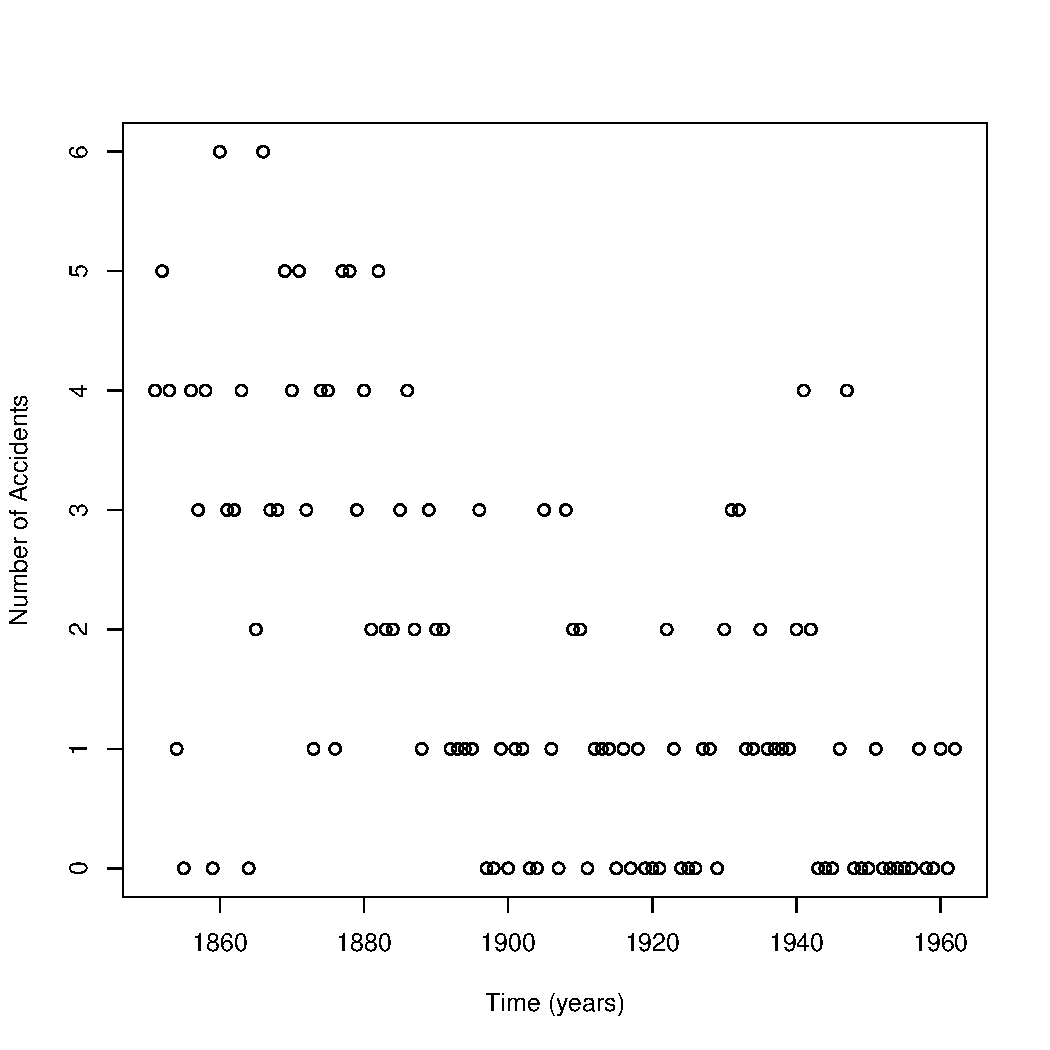
\includegraphics[width=0.6\textwidth]{images/coal.pdf}

\end{frame}


\begin{frame}[fragile]
\frametitle{Change-Point Model: Priors}
We will use log-uniform priors for $\lambda_1$ and $\lambda_2$ independently.
\begin{minted}{r}
log_lambda1 ~ dunif(-10, 10)
lambda1 <- exp(log_lambda1)

log_lambda2 ~ dunif(-10, 10)
lambda2 <- exp(log_lambda2)
\end{minted}
\pause
Note: Distributions will be independent if, when defining one, you
make no reference to another node on the right hand side.

\end{frame}

\begin{frame}[fragile]
\frametitle{Change-Point Model: Priors}
We will use a uniform prior for the change year, $t_c$, between the
endpoints of the data.
\begin{minted}{r}
t_c ~ dunif(1851, 1962)
\end{minted}
\pause

{\bf Note:}
While it might look like we are defining a prior based on the data,
which is not technically valid, we are actually not. The time values
in the data are prior information, not data, as they have no sampling
distribution --- our whole calculation is conditional on it already.

\end{frame}


\begin{frame}[fragile]
\frametitle{Change-Point Model: Sampling Distribution}
To construct the sampling distribution we will use \mintinline{r}{step()}
which is like R's \mintinline{r}{ifelse()}. It returns 0 if the argument is
negative and 1 otherwise.

\begin{minted}{r}
for(i in 1:N)
{
    mu[i] <- lambda1 + step(t[i] - t_c)*(lambda2 - lambda1)
    y[i] ~ dpois(mu[i])
}
\end{minted}
\pause

We could have done this in one line, without defining \mintinline{r}{mu}
first.

\end{frame}

\begin{frame}
\frametitle{Main Result: Marginal Posterior for $t_c$}
\begin{center}
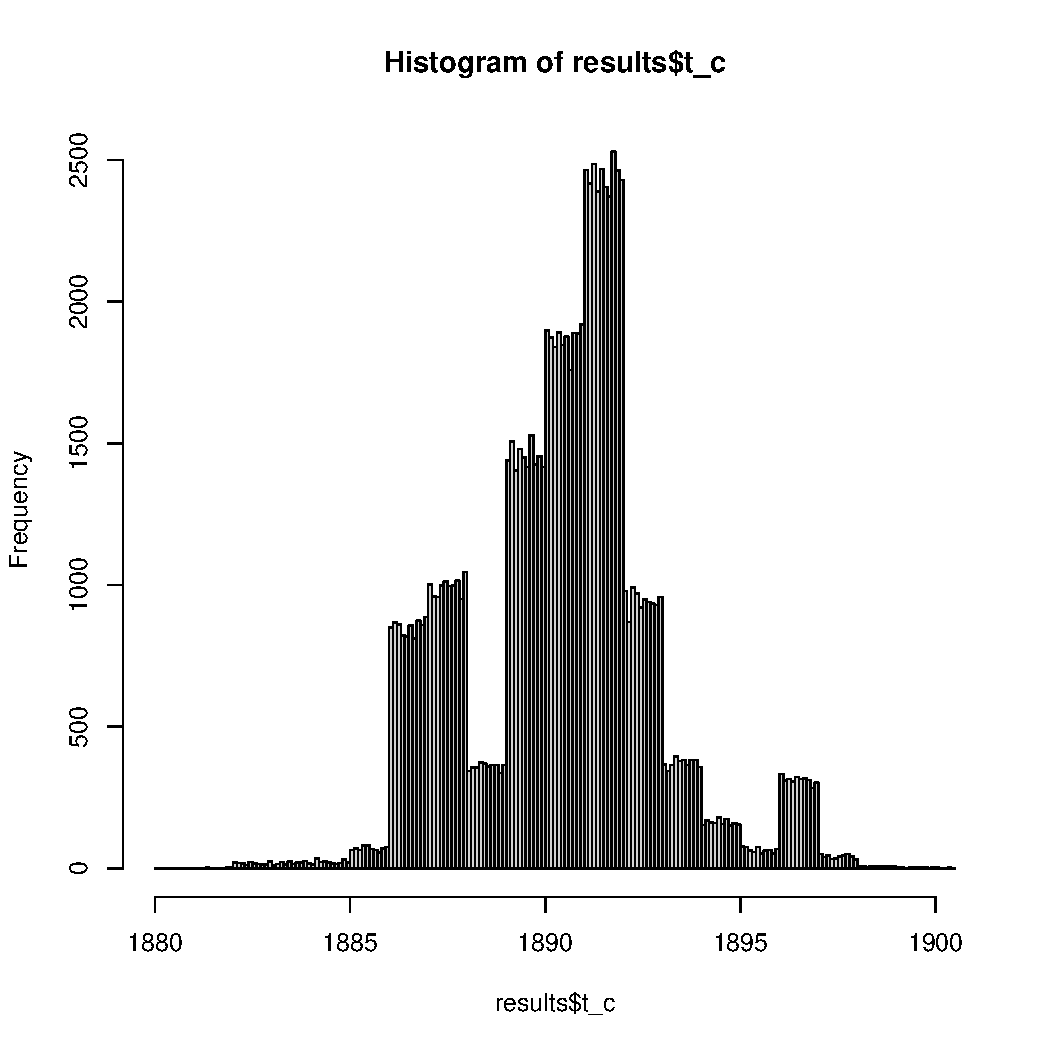
\includegraphics[width=0.6\textwidth]{images/coal_posterior.pdf} \\
\end{center}
Why is it uniform between the years?

\end{frame}


\begin{frame}[fragile]
\frametitle{Lines Through the Data}
In regression problems like this, it is often nice to plot
some model lines, with parameters representative of the
posterior distribution, through the data.
\begin{minted}{r}
plot(data$t, data$y)
cols = 3:114 # A bit annoying to find
rows = sample(1:nrow(results), 10)
mu = results[rows, cols]
for(i in 1:nrow(mu))
    lines(data$t, mu[i, ])
\end{minted}

\end{frame}

\begin{frame}
\frametitle{Lines Through the Data}
\begin{center}
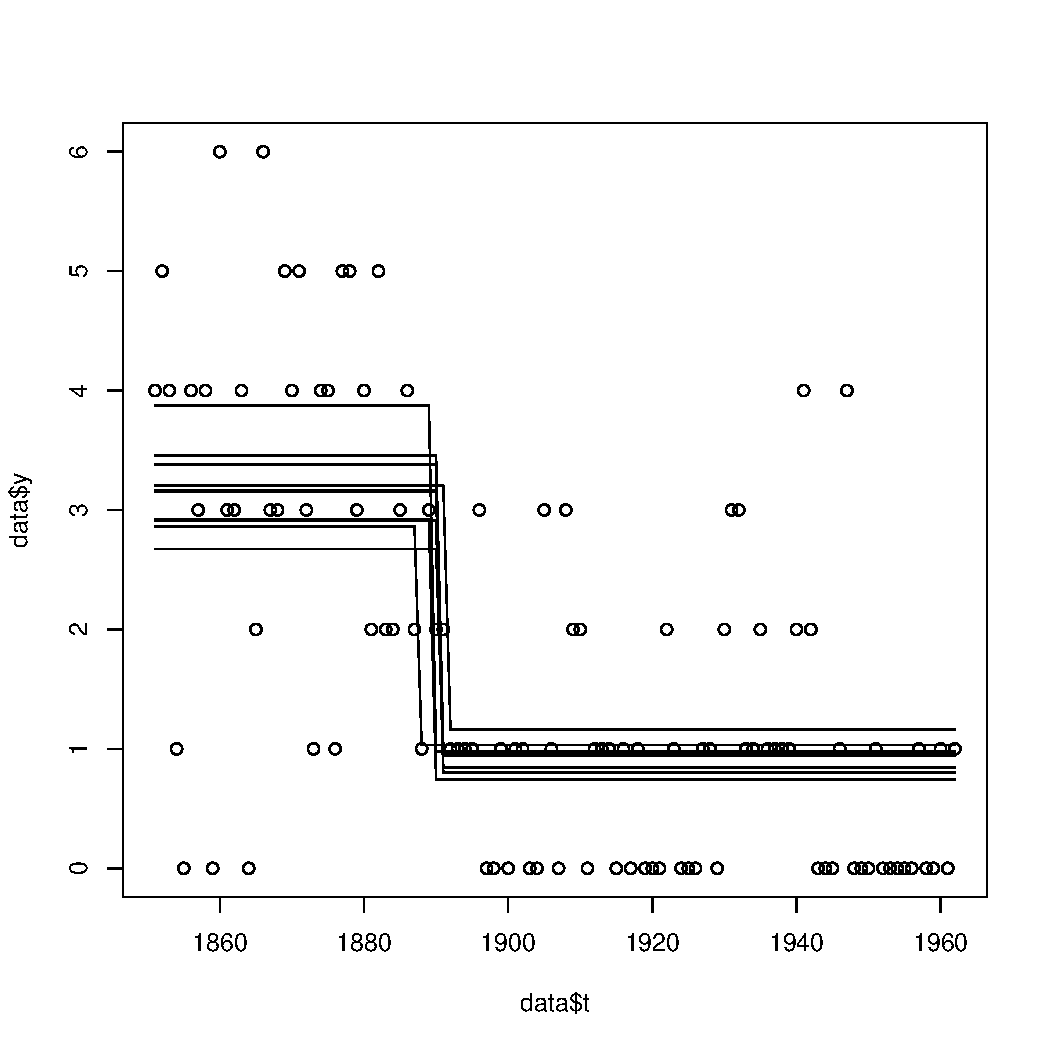
\includegraphics[width=0.6\textwidth]{images/coal_lines.pdf} \\
\end{center}
Why is it uniform between the years?

\end{frame}


\begin{frame}[fragile]
\frametitle{Summaries}
Let's summarise the posterior for $t_c$. Some are easy:

\begin{minted}{r}
> mean(results$t_c)
[1] 1890.447
> sd(results$t_c)
[1] 2.438453
\end{minted}

\end{frame}

\begin{frame}[fragile]
\frametitle{Summaries}
Let's compute a 95\% credible interval. There are two ways:

\begin{minted}{r}
sorted = sort(results$t_c)
left = sorted[0.025*length(sorted)]
right = sorted[0.975*length(sorted)]
\end{minted}

The result is:
\begin{minted}{r}
> left
[1] 1886.137
> right
[1] 1896.395
\end{minted}

\end{frame}


\begin{frame}[fragile]
\frametitle{Summaries}
Let's compute a 95\% credible interval. This is the easier way:
\begin{minted}{r}
interval = quantile(results$t_c, probs=c(0.025, 0.975))
left = interval[1]
right = interval[2]
\end{minted}

\end{frame}


\begin{frame}[fragile]
\frametitle{Plotting the Interval}
\begin{minted}{r}
hist(results$t_c, breaks=200)
abline(v=left)
abline(v=right)
\end{minted}

\end{frame}

\begin{frame}[fragile]
\frametitle{Plotting the Interval}
\centering
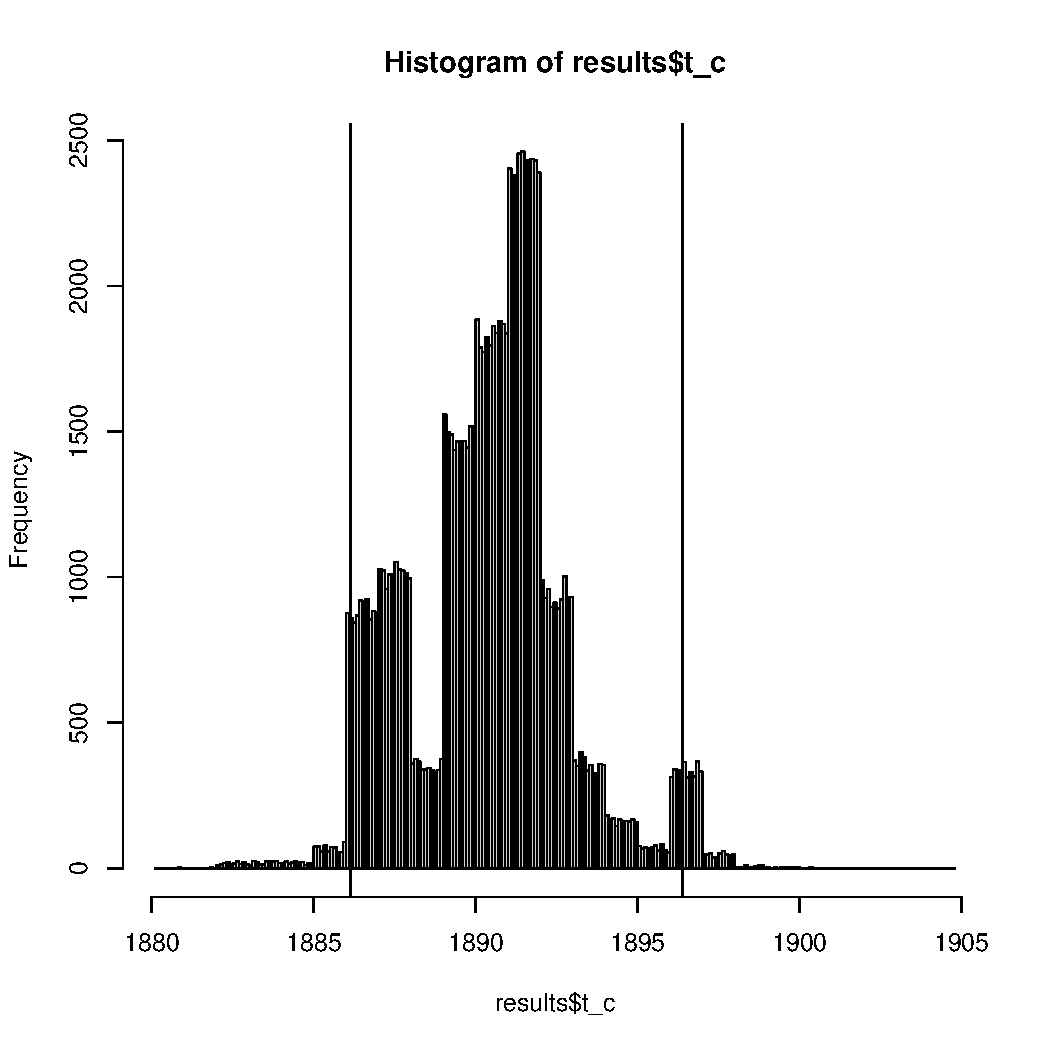
\includegraphics[width=0.6\textwidth]{images/coal_interval.pdf}

\end{frame}


\begin{frame}
\frametitle{What's Coming Next}
Now that we can use MCMC to compute our posterior distributions,
we can enlarge our models to multiple parameters. We will
require more careful thinking about our priors,
which can have unintended consequences in high dimensions.

\pause
We will soon look at hierarchical models, which are important
when you have many unknown parameters of the same `type'.
These arise frequently in genomics (I am assured).

\end{frame}

\end{document}

